\documentclass{article}
\usepackage{geometry,color,graphicx}
\usepackage{caption}
\usepackage{subcaption}
\usepackage{float}


\begin{document}

\title{Project 1: Derivatives and Simple Harmonic Oscillators}

\author{Gabriel Smadi\\
  College of Engineering, \\
  Physics Department, \\
  Syracuse University,\\
  \texttt{gsmadi@syr.edu}}
\maketitle

\begin{abstract}
\end{abstract}

\section{Introduction}

\section{Numerical derivative}
By definition of the derivative,


\begin{table}[H]
  \begin{center}
    \begin{tabular}{|c|c|c|c|}
      \hline
      x & Computed & Actual & Error \\
      \hline
      \( 0 \) & -0.191785 & 1.000000 & -1.191785 \\
      \hline
      \( \frac{\pi}{8} \) & -0.232012 & 0.923880 & -1.155892 \\
      \hline
      \( \frac{\pi}{4} \) & -0.236918 & 0.707107 & -0.944025 \\
      \hline
      \( \frac{3 \pi}{8} \) & -0.205755 & 0.382683 & -0.588438 \\
      \hline
      \( \frac{\pi}{2} \) & -0.143268 & 0.000000 & -0.143267 \\
      \hline
      \( \frac{5 \pi}{8} \) & -0.058969 & -0.382684 & 0.323714 \\
      \hline
      \( \frac{3 \pi}{4} \) & 0.034307 & -0.707107 & 0.741414 \\
      \hline
      \( \frac{7 \pi}{8} \) & 0.122360 & -0.923880 & 1.046239 \\
      \hline
      \( \pi \) & 0.191785 & -1.000000 & 1.191785 \\
      \hline
    \end{tabular}
  \end{center}
  \caption {Computed and actual values of \( \frac{d \sin(x)}{dx} \) for $h=5.0$}
  \label{table:comparison}
\end{table}


\begin{figure}[H]
  \begin{center}
    \scalebox{.8}{% GNUPLOT: LaTeX picture with Postscript
\begingroup
  \makeatletter
  \providecommand\color[2][]{%
    \GenericError{(gnuplot) \space\space\space\@spaces}{%
      Package color not loaded in conjunction with
      terminal option `colourtext'%
    }{See the gnuplot documentation for explanation.%
    }{Either use 'blacktext' in gnuplot or load the package
      color.sty in LaTeX.}%
    \renewcommand\color[2][]{}%
  }%
  \providecommand\includegraphics[2][]{%
    \GenericError{(gnuplot) \space\space\space\@spaces}{%
      Package graphicx or graphics not loaded%
    }{See the gnuplot documentation for explanation.%
    }{The gnuplot epslatex terminal needs graphicx.sty or graphics.sty.}%
    \renewcommand\includegraphics[2][]{}%
  }%
  \providecommand\rotatebox[2]{#2}%
  \@ifundefined{ifGPcolor}{%
    \newif\ifGPcolor
    \GPcolortrue
  }{}%
  \@ifundefined{ifGPblacktext}{%
    \newif\ifGPblacktext
    \GPblacktextfalse
  }{}%
  % define a \g@addto@macro without @ in the name:
  \let\gplgaddtomacro\g@addto@macro
  % define empty templates for all commands taking text:
  \gdef\gplbacktext{}%
  \gdef\gplfronttext{}%
  \makeatother
  \ifGPblacktext
    % no textcolor at all
    \def\colorrgb#1{}%
    \def\colorgray#1{}%
  \else
    % gray or color?
    \ifGPcolor
      \def\colorrgb#1{\color[rgb]{#1}}%
      \def\colorgray#1{\color[gray]{#1}}%
      \expandafter\def\csname LTw\endcsname{\color{white}}%
      \expandafter\def\csname LTb\endcsname{\color{black}}%
      \expandafter\def\csname LTa\endcsname{\color{black}}%
      \expandafter\def\csname LT0\endcsname{\color[rgb]{1,0,0}}%
      \expandafter\def\csname LT1\endcsname{\color[rgb]{0,1,0}}%
      \expandafter\def\csname LT2\endcsname{\color[rgb]{0,0,1}}%
      \expandafter\def\csname LT3\endcsname{\color[rgb]{1,0,1}}%
      \expandafter\def\csname LT4\endcsname{\color[rgb]{0,1,1}}%
      \expandafter\def\csname LT5\endcsname{\color[rgb]{1,1,0}}%
      \expandafter\def\csname LT6\endcsname{\color[rgb]{0,0,0}}%
      \expandafter\def\csname LT7\endcsname{\color[rgb]{1,0.3,0}}%
      \expandafter\def\csname LT8\endcsname{\color[rgb]{0.5,0.5,0.5}}%
    \else
      % gray
      \def\colorrgb#1{\color{black}}%
      \def\colorgray#1{\color[gray]{#1}}%
      \expandafter\def\csname LTw\endcsname{\color{white}}%
      \expandafter\def\csname LTb\endcsname{\color{black}}%
      \expandafter\def\csname LTa\endcsname{\color{black}}%
      \expandafter\def\csname LT0\endcsname{\color{black}}%
      \expandafter\def\csname LT1\endcsname{\color{black}}%
      \expandafter\def\csname LT2\endcsname{\color{black}}%
      \expandafter\def\csname LT3\endcsname{\color{black}}%
      \expandafter\def\csname LT4\endcsname{\color{black}}%
      \expandafter\def\csname LT5\endcsname{\color{black}}%
      \expandafter\def\csname LT6\endcsname{\color{black}}%
      \expandafter\def\csname LT7\endcsname{\color{black}}%
      \expandafter\def\csname LT8\endcsname{\color{black}}%
    \fi
  \fi
    \setlength{\unitlength}{0.0500bp}%
    \ifx\gptboxheight\undefined%
      \newlength{\gptboxheight}%
      \newlength{\gptboxwidth}%
      \newsavebox{\gptboxtext}%
    \fi%
    \setlength{\fboxrule}{0.5pt}%
    \setlength{\fboxsep}{1pt}%
\begin{picture}(6480.00,5212.00)%
    \gplgaddtomacro\gplbacktext{%
      \csname LTb\endcsname%
      \put(946,704){\makebox(0,0)[r]{\strut{}$-1$}}%
      \csname LTb\endcsname%
      \put(946,1721){\makebox(0,0)[r]{\strut{}$-0.5$}}%
      \csname LTb\endcsname%
      \put(946,2738){\makebox(0,0)[r]{\strut{}$0$}}%
      \csname LTb\endcsname%
      \put(946,3754){\makebox(0,0)[r]{\strut{}$0.5$}}%
      \csname LTb\endcsname%
      \put(946,4771){\makebox(0,0)[r]{\strut{}$1$}}%
      \csname LTb\endcsname%
      \put(1078,484){\makebox(0,0){\strut{}$0$}}%
      \csname LTb\endcsname%
      \put(2329,484){\makebox(0,0){\strut{}$\frac{\pi}{4}$}}%
      \csname LTb\endcsname%
      \put(3581,484){\makebox(0,0){\strut{}$\frac{\pi}{2}$}}%
      \csname LTb\endcsname%
      \put(4832,484){\makebox(0,0){\strut{}$\frac{3 \pi}{4}$}}%
      \csname LTb\endcsname%
      \put(6083,484){\makebox(0,0){\strut{}$\pi$}}%
    }%
    \gplgaddtomacro\gplfronttext{%
      \csname LTb\endcsname%
      \put(176,2737){\rotatebox{-270}{\makebox(0,0){\strut{}y}}}%
      \put(3580,154){\makebox(0,0){\strut{}x}}%
      \put(3580,5101){\makebox(0,0){\strut{}Actual vs. Computed derivative}}%
      \csname LTb\endcsname%
      \put(5096,4598){\makebox(0,0)[r]{\strut{}Computed with $h=5.0$}}%
      \csname LTb\endcsname%
      \put(5096,4378){\makebox(0,0)[r]{\strut{}Computed with $h=0.5$}}%
      \csname LTb\endcsname%
      \put(5096,4158){\makebox(0,0)[r]{\strut{}Computed with $h=0.5$}}%
      \csname LTb\endcsname%
      \put(5096,3938){\makebox(0,0)[r]{\strut{}Actual}}%
    }%
    \gplbacktext
    \put(0,0){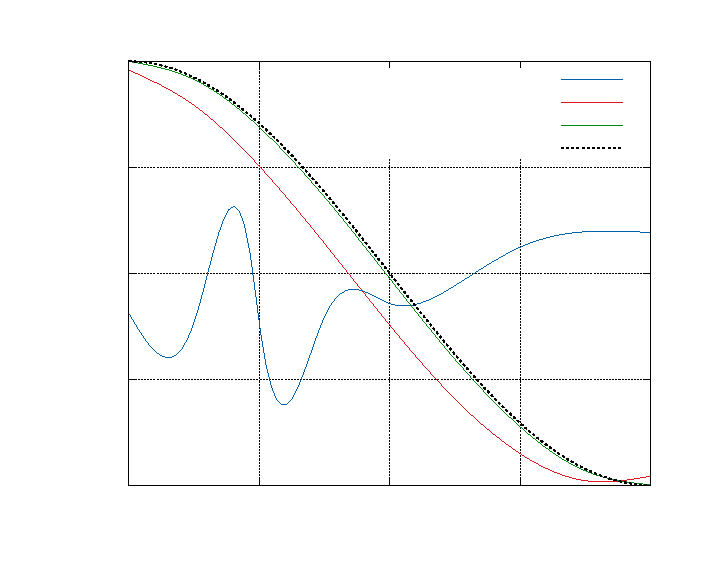
\includegraphics{actual_computed}}%
    \gplfronttext
  \end{picture}%
\endgroup
}
  \end{center}
  \caption{Actual vs. Computed derivatives for different $h$}
  \label{fig:actual_computed}
\end{figure}

From Figure \ref{fig:derivative}, the error of our computed value can be seen as a function of $x$. We can see in the
graph how the errors converge to 0 as $h \to 0$.

\begin{figure}[H]
  \begin{center}
    \scalebox{.8}{% GNUPLOT: LaTeX picture with Postscript
\begingroup
  \makeatletter
  \providecommand\color[2][]{%
    \GenericError{(gnuplot) \space\space\space\@spaces}{%
      Package color not loaded in conjunction with
      terminal option `colourtext'%
    }{See the gnuplot documentation for explanation.%
    }{Either use 'blacktext' in gnuplot or load the package
      color.sty in LaTeX.}%
    \renewcommand\color[2][]{}%
  }%
  \providecommand\includegraphics[2][]{%
    \GenericError{(gnuplot) \space\space\space\@spaces}{%
      Package graphicx or graphics not loaded%
    }{See the gnuplot documentation for explanation.%
    }{The gnuplot epslatex terminal needs graphicx.sty or graphics.sty.}%
    \renewcommand\includegraphics[2][]{}%
  }%
  \providecommand\rotatebox[2]{#2}%
  \@ifundefined{ifGPcolor}{%
    \newif\ifGPcolor
    \GPcolortrue
  }{}%
  \@ifundefined{ifGPblacktext}{%
    \newif\ifGPblacktext
    \GPblacktextfalse
  }{}%
  % define a \g@addto@macro without @ in the name:
  \let\gplgaddtomacro\g@addto@macro
  % define empty templates for all commands taking text:
  \gdef\gplbacktext{}%
  \gdef\gplfronttext{}%
  \makeatother
  \ifGPblacktext
    % no textcolor at all
    \def\colorrgb#1{}%
    \def\colorgray#1{}%
  \else
    % gray or color?
    \ifGPcolor
      \def\colorrgb#1{\color[rgb]{#1}}%
      \def\colorgray#1{\color[gray]{#1}}%
      \expandafter\def\csname LTw\endcsname{\color{white}}%
      \expandafter\def\csname LTb\endcsname{\color{black}}%
      \expandafter\def\csname LTa\endcsname{\color{black}}%
      \expandafter\def\csname LT0\endcsname{\color[rgb]{1,0,0}}%
      \expandafter\def\csname LT1\endcsname{\color[rgb]{0,1,0}}%
      \expandafter\def\csname LT2\endcsname{\color[rgb]{0,0,1}}%
      \expandafter\def\csname LT3\endcsname{\color[rgb]{1,0,1}}%
      \expandafter\def\csname LT4\endcsname{\color[rgb]{0,1,1}}%
      \expandafter\def\csname LT5\endcsname{\color[rgb]{1,1,0}}%
      \expandafter\def\csname LT6\endcsname{\color[rgb]{0,0,0}}%
      \expandafter\def\csname LT7\endcsname{\color[rgb]{1,0.3,0}}%
      \expandafter\def\csname LT8\endcsname{\color[rgb]{0.5,0.5,0.5}}%
    \else
      % gray
      \def\colorrgb#1{\color{black}}%
      \def\colorgray#1{\color[gray]{#1}}%
      \expandafter\def\csname LTw\endcsname{\color{white}}%
      \expandafter\def\csname LTb\endcsname{\color{black}}%
      \expandafter\def\csname LTa\endcsname{\color{black}}%
      \expandafter\def\csname LT0\endcsname{\color{black}}%
      \expandafter\def\csname LT1\endcsname{\color{black}}%
      \expandafter\def\csname LT2\endcsname{\color{black}}%
      \expandafter\def\csname LT3\endcsname{\color{black}}%
      \expandafter\def\csname LT4\endcsname{\color{black}}%
      \expandafter\def\csname LT5\endcsname{\color{black}}%
      \expandafter\def\csname LT6\endcsname{\color{black}}%
      \expandafter\def\csname LT7\endcsname{\color{black}}%
      \expandafter\def\csname LT8\endcsname{\color{black}}%
    \fi
  \fi
    \setlength{\unitlength}{0.0500bp}%
    \ifx\gptboxheight\undefined%
      \newlength{\gptboxheight}%
      \newlength{\gptboxwidth}%
      \newsavebox{\gptboxtext}%
    \fi%
    \setlength{\fboxrule}{0.5pt}%
    \setlength{\fboxsep}{1pt}%
\begin{picture}(6480.00,5212.00)%
    \gplgaddtomacro\gplbacktext{%
      \csname LTb\endcsname%
      \put(682,704){\makebox(0,0)[r]{\strut{}$-4$}}%
      \csname LTb\endcsname%
      \put(682,1285){\makebox(0,0)[r]{\strut{}$-3$}}%
      \csname LTb\endcsname%
      \put(682,1866){\makebox(0,0)[r]{\strut{}$-2$}}%
      \csname LTb\endcsname%
      \put(682,2447){\makebox(0,0)[r]{\strut{}$-1$}}%
      \csname LTb\endcsname%
      \put(682,3028){\makebox(0,0)[r]{\strut{}$0$}}%
      \csname LTb\endcsname%
      \put(682,3609){\makebox(0,0)[r]{\strut{}$1$}}%
      \csname LTb\endcsname%
      \put(682,4190){\makebox(0,0)[r]{\strut{}$2$}}%
      \csname LTb\endcsname%
      \put(682,4771){\makebox(0,0)[r]{\strut{}$3$}}%
      \csname LTb\endcsname%
      \put(814,484){\makebox(0,0){\strut{}$0$}}%
      \csname LTb\endcsname%
      \put(2131,484){\makebox(0,0){\strut{}$\frac{\pi}{4}$}}%
      \csname LTb\endcsname%
      \put(3449,484){\makebox(0,0){\strut{}$\frac{\pi}{2}$}}%
      \csname LTb\endcsname%
      \put(4766,484){\makebox(0,0){\strut{}$\frac{3 \pi}{4}$}}%
      \csname LTb\endcsname%
      \put(6083,484){\makebox(0,0){\strut{}$\pi$}}%
    }%
    \gplgaddtomacro\gplfronttext{%
      \csname LTb\endcsname%
      \put(176,2737){\rotatebox{-270}{\makebox(0,0){\strut{}Error}}}%
      \put(3448,154){\makebox(0,0){\strut{}x}}%
      \put(3448,5101){\makebox(0,0){\strut{}Errors}}%
      \csname LTb\endcsname%
      \put(5096,4598){\makebox(0,0)[r]{\strut{}$h=5.0$}}%
      \csname LTb\endcsname%
      \put(5096,4378){\makebox(0,0)[r]{\strut{}$h=0.5$}}%
      \csname LTb\endcsname%
      \put(5096,4158){\makebox(0,0)[r]{\strut{}$h=0.05$}}%
    }%
    \gplbacktext
    \put(0,0){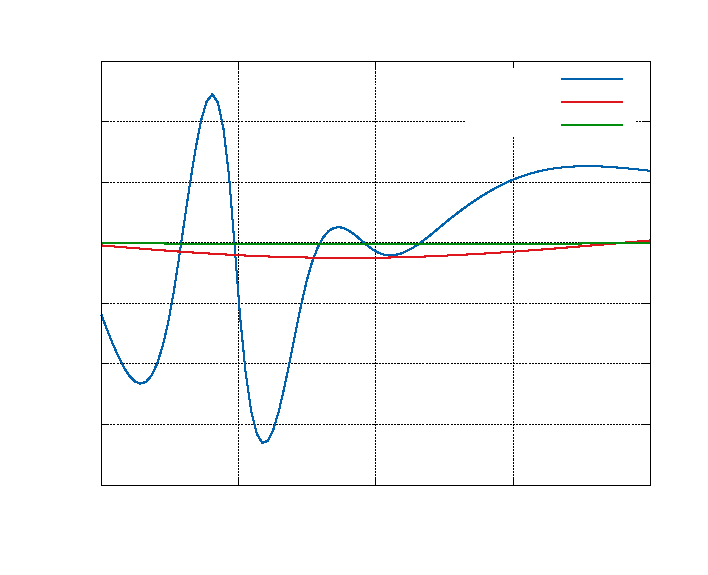
\includegraphics{derivative}}%
    \gplfronttext
  \end{picture}%
\endgroup
}
  \end{center}
  \caption{Convergence of errors as $h\to 0$}
  \label{fig:derivative}
\end{figure}

In Figure \ref{fig:errors}, we see the magnitude of our errors as a function of $h$. To no
surprise, it is clear that as $h \to 0$ our errors $err(h) \to 0$.Note that for greater
$h$ the errors may appear to oscillate. This is due to the periodic nature of the functions we are
investigating. However, rest assured that as we minimize $h$ to $0$ we will automatically minimize
our errors $err(h)$.

\begin{figure}[H]
  \begin{center}
    \scalebox{.8}{% GNUPLOT: LaTeX picture with Postscript
\begingroup
  \makeatletter
  \providecommand\color[2][]{%
    \GenericError{(gnuplot) \space\space\space\@spaces}{%
      Package color not loaded in conjunction with
      terminal option `colourtext'%
    }{See the gnuplot documentation for explanation.%
    }{Either use 'blacktext' in gnuplot or load the package
      color.sty in LaTeX.}%
    \renewcommand\color[2][]{}%
  }%
  \providecommand\includegraphics[2][]{%
    \GenericError{(gnuplot) \space\space\space\@spaces}{%
      Package graphicx or graphics not loaded%
    }{See the gnuplot documentation for explanation.%
    }{The gnuplot epslatex terminal needs graphicx.sty or graphics.sty.}%
    \renewcommand\includegraphics[2][]{}%
  }%
  \providecommand\rotatebox[2]{#2}%
  \@ifundefined{ifGPcolor}{%
    \newif\ifGPcolor
    \GPcolortrue
  }{}%
  \@ifundefined{ifGPblacktext}{%
    \newif\ifGPblacktext
    \GPblacktextfalse
  }{}%
  % define a \g@addto@macro without @ in the name:
  \let\gplgaddtomacro\g@addto@macro
  % define empty templates for all commands taking text:
  \gdef\gplbacktext{}%
  \gdef\gplfronttext{}%
  \makeatother
  \ifGPblacktext
    % no textcolor at all
    \def\colorrgb#1{}%
    \def\colorgray#1{}%
  \else
    % gray or color?
    \ifGPcolor
      \def\colorrgb#1{\color[rgb]{#1}}%
      \def\colorgray#1{\color[gray]{#1}}%
      \expandafter\def\csname LTw\endcsname{\color{white}}%
      \expandafter\def\csname LTb\endcsname{\color{black}}%
      \expandafter\def\csname LTa\endcsname{\color{black}}%
      \expandafter\def\csname LT0\endcsname{\color[rgb]{1,0,0}}%
      \expandafter\def\csname LT1\endcsname{\color[rgb]{0,1,0}}%
      \expandafter\def\csname LT2\endcsname{\color[rgb]{0,0,1}}%
      \expandafter\def\csname LT3\endcsname{\color[rgb]{1,0,1}}%
      \expandafter\def\csname LT4\endcsname{\color[rgb]{0,1,1}}%
      \expandafter\def\csname LT5\endcsname{\color[rgb]{1,1,0}}%
      \expandafter\def\csname LT6\endcsname{\color[rgb]{0,0,0}}%
      \expandafter\def\csname LT7\endcsname{\color[rgb]{1,0.3,0}}%
      \expandafter\def\csname LT8\endcsname{\color[rgb]{0.5,0.5,0.5}}%
    \else
      % gray
      \def\colorrgb#1{\color{black}}%
      \def\colorgray#1{\color[gray]{#1}}%
      \expandafter\def\csname LTw\endcsname{\color{white}}%
      \expandafter\def\csname LTb\endcsname{\color{black}}%
      \expandafter\def\csname LTa\endcsname{\color{black}}%
      \expandafter\def\csname LT0\endcsname{\color{black}}%
      \expandafter\def\csname LT1\endcsname{\color{black}}%
      \expandafter\def\csname LT2\endcsname{\color{black}}%
      \expandafter\def\csname LT3\endcsname{\color{black}}%
      \expandafter\def\csname LT4\endcsname{\color{black}}%
      \expandafter\def\csname LT5\endcsname{\color{black}}%
      \expandafter\def\csname LT6\endcsname{\color{black}}%
      \expandafter\def\csname LT7\endcsname{\color{black}}%
      \expandafter\def\csname LT8\endcsname{\color{black}}%
    \fi
  \fi
    \setlength{\unitlength}{0.0500bp}%
    \ifx\gptboxheight\undefined%
      \newlength{\gptboxheight}%
      \newlength{\gptboxwidth}%
      \newsavebox{\gptboxtext}%
    \fi%
    \setlength{\fboxrule}{0.5pt}%
    \setlength{\fboxsep}{1pt}%
\begin{picture}(6480.00,5212.00)%
    \gplgaddtomacro\gplbacktext{%
      \csname LTb\endcsname%
      \put(814,704){\makebox(0,0)[r]{\strut{}$0$}}%
      \csname LTb\endcsname%
      \put(814,1285){\makebox(0,0)[r]{\strut{}$0.2$}}%
      \csname LTb\endcsname%
      \put(814,1866){\makebox(0,0)[r]{\strut{}$0.4$}}%
      \csname LTb\endcsname%
      \put(814,2447){\makebox(0,0)[r]{\strut{}$0.6$}}%
      \csname LTb\endcsname%
      \put(814,3028){\makebox(0,0)[r]{\strut{}$0.8$}}%
      \csname LTb\endcsname%
      \put(814,3609){\makebox(0,0)[r]{\strut{}$1$}}%
      \csname LTb\endcsname%
      \put(814,4190){\makebox(0,0)[r]{\strut{}$1.2$}}%
      \csname LTb\endcsname%
      \put(814,4771){\makebox(0,0)[r]{\strut{}$1.4$}}%
      \csname LTb\endcsname%
      \put(946,484){\makebox(0,0){\strut{}$0$}}%
      \csname LTb\endcsname%
      \put(1460,484){\makebox(0,0){\strut{}$0.5$}}%
      \csname LTb\endcsname%
      \put(1973,484){\makebox(0,0){\strut{}$1$}}%
      \csname LTb\endcsname%
      \put(2487,484){\makebox(0,0){\strut{}$1.5$}}%
      \csname LTb\endcsname%
      \put(3001,484){\makebox(0,0){\strut{}$2$}}%
      \csname LTb\endcsname%
      \put(3515,484){\makebox(0,0){\strut{}$2.5$}}%
      \csname LTb\endcsname%
      \put(4028,484){\makebox(0,0){\strut{}$3$}}%
      \csname LTb\endcsname%
      \put(4542,484){\makebox(0,0){\strut{}$3.5$}}%
      \csname LTb\endcsname%
      \put(5056,484){\makebox(0,0){\strut{}$4$}}%
      \csname LTb\endcsname%
      \put(5569,484){\makebox(0,0){\strut{}$4.5$}}%
      \csname LTb\endcsname%
      \put(6083,484){\makebox(0,0){\strut{}$5$}}%
    }%
    \gplgaddtomacro\gplfronttext{%
      \csname LTb\endcsname%
      \put(176,2737){\rotatebox{-270}{\makebox(0,0){\strut{}Error}}}%
      \put(3514,154){\makebox(0,0){\strut{}h}}%
      \put(3514,5101){\makebox(0,0){\strut{}Errors vs. h}}%
      \csname LTb\endcsname%
      \put(5096,4598){\makebox(0,0)[r]{\strut{}$x=0$}}%
      \csname LTb\endcsname%
      \put(5096,4378){\makebox(0,0)[r]{\strut{}$x=\frac{\pi}{4}$}}%
      \csname LTb\endcsname%
      \put(5096,4158){\makebox(0,0)[r]{\strut{}$x=\frac{\pi}{2}$}}%
      \csname LTb\endcsname%
      \put(5096,3938){\makebox(0,0)[r]{\strut{}$x=\frac{3 \pi}{4}$}}%
      \csname LTb\endcsname%
      \put(5096,3718){\makebox(0,0)[r]{\strut{}$x=\pi$}}%
    }%
    \gplbacktext
    \put(0,0){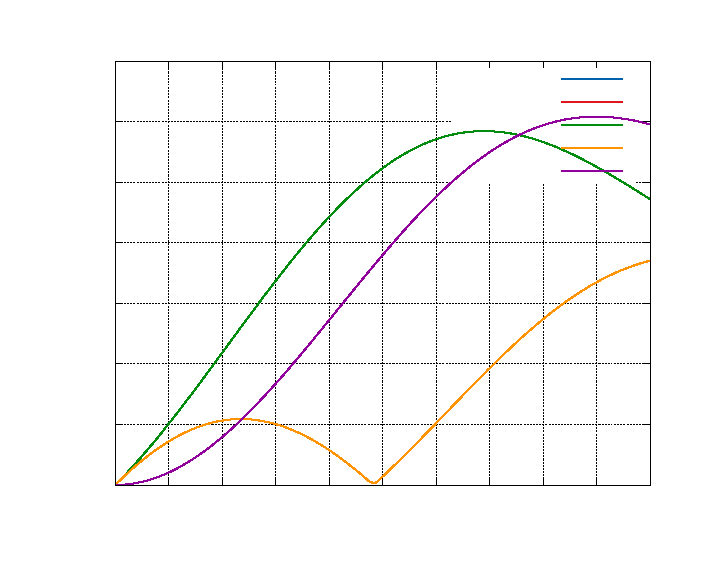
\includegraphics{plots/errors}}%
    \gplfronttext
  \end{picture}%
\endgroup
}
  \end{center}
  \caption{Errors as a function of $h$}
  \label{fig:errors}
\end{figure}

For our purposes, floats are more that sufficient for the precision we require. However, for greater
precision doubles would be used. Doubles can hold 15 decimal places as compared to floats, which can
only hold 7. Thus, by using doubles instead of floats we could get much more precision. But in our situation,
there would not be much of an advantage. We can further minimize our errors, but for big $h$ those errors shall
still remain either way.


\section{Simple Harmonic Oscillator}

The most common expressions for a simple harmonic oscillator are given below,

\begin{equation} \label{eq:2}
x(t)=B\cos(\omega t)
\end{equation}

\begin{equation} \label{eq:3}
v(t)=-\omega B\cos(\omega t)
\end{equation}

\begin{equation} \label{eq:4}
a(t)=-\omega^2 B\cos(\omega t)
\end{equation}

Below in Figure \ref{fig:sho}, we take a different approach to investigate a simple harmonic
oscillator. In the plots we investigate the relationship of the acceleration and velocity of
the SHO against its displacement. In other words, the acceleration $a$  and velocity $v$ as a function
of position $x$. For even small $n$, it is apparent the linear relationship of the acceleration to
the position. However, for the velocity the relationship is not quite clear.

\begin{figure}[H]
    \centering
    \begin{subfigure}[b]{0.35\textwidth}
        \scalebox{.8}{% GNUPLOT: LaTeX picture with Postscript
\begingroup
  \makeatletter
  \providecommand\color[2][]{%
    \GenericError{(gnuplot) \space\space\space\@spaces}{%
      Package color not loaded in conjunction with
      terminal option `colourtext'%
    }{See the gnuplot documentation for explanation.%
    }{Either use 'blacktext' in gnuplot or load the package
      color.sty in LaTeX.}%
    \renewcommand\color[2][]{}%
  }%
  \providecommand\includegraphics[2][]{%
    \GenericError{(gnuplot) \space\space\space\@spaces}{%
      Package graphicx or graphics not loaded%
    }{See the gnuplot documentation for explanation.%
    }{The gnuplot epslatex terminal needs graphicx.sty or graphics.sty.}%
    \renewcommand\includegraphics[2][]{}%
  }%
  \providecommand\rotatebox[2]{#2}%
  \@ifundefined{ifGPcolor}{%
    \newif\ifGPcolor
    \GPcolortrue
  }{}%
  \@ifundefined{ifGPblacktext}{%
    \newif\ifGPblacktext
    \GPblacktextfalse
  }{}%
  % define a \g@addto@macro without @ in the name:
  \let\gplgaddtomacro\g@addto@macro
  % define empty templates for all commands taking text:
  \gdef\gplbacktext{}%
  \gdef\gplfronttext{}%
  \makeatother
  \ifGPblacktext
    % no textcolor at all
    \def\colorrgb#1{}%
    \def\colorgray#1{}%
  \else
    % gray or color?
    \ifGPcolor
      \def\colorrgb#1{\color[rgb]{#1}}%
      \def\colorgray#1{\color[gray]{#1}}%
      \expandafter\def\csname LTw\endcsname{\color{white}}%
      \expandafter\def\csname LTb\endcsname{\color{black}}%
      \expandafter\def\csname LTa\endcsname{\color{black}}%
      \expandafter\def\csname LT0\endcsname{\color[rgb]{1,0,0}}%
      \expandafter\def\csname LT1\endcsname{\color[rgb]{0,1,0}}%
      \expandafter\def\csname LT2\endcsname{\color[rgb]{0,0,1}}%
      \expandafter\def\csname LT3\endcsname{\color[rgb]{1,0,1}}%
      \expandafter\def\csname LT4\endcsname{\color[rgb]{0,1,1}}%
      \expandafter\def\csname LT5\endcsname{\color[rgb]{1,1,0}}%
      \expandafter\def\csname LT6\endcsname{\color[rgb]{0,0,0}}%
      \expandafter\def\csname LT7\endcsname{\color[rgb]{1,0.3,0}}%
      \expandafter\def\csname LT8\endcsname{\color[rgb]{0.5,0.5,0.5}}%
    \else
      % gray
      \def\colorrgb#1{\color{black}}%
      \def\colorgray#1{\color[gray]{#1}}%
      \expandafter\def\csname LTw\endcsname{\color{white}}%
      \expandafter\def\csname LTb\endcsname{\color{black}}%
      \expandafter\def\csname LTa\endcsname{\color{black}}%
      \expandafter\def\csname LT0\endcsname{\color{black}}%
      \expandafter\def\csname LT1\endcsname{\color{black}}%
      \expandafter\def\csname LT2\endcsname{\color{black}}%
      \expandafter\def\csname LT3\endcsname{\color{black}}%
      \expandafter\def\csname LT4\endcsname{\color{black}}%
      \expandafter\def\csname LT5\endcsname{\color{black}}%
      \expandafter\def\csname LT6\endcsname{\color{black}}%
      \expandafter\def\csname LT7\endcsname{\color{black}}%
      \expandafter\def\csname LT8\endcsname{\color{black}}%
    \fi
  \fi
    \setlength{\unitlength}{0.0500bp}%
    \ifx\gptboxheight\undefined%
      \newlength{\gptboxheight}%
      \newlength{\gptboxwidth}%
      \newsavebox{\gptboxtext}%
    \fi%
    \setlength{\fboxrule}{0.5pt}%
    \setlength{\fboxsep}{1pt}%
\begin{picture}(4320.00,3600.00)%
    \gplgaddtomacro\gplbacktext{%
      \csname LTb\endcsname%
      \put(946,704){\makebox(0,0)[r]{\strut{}$-2$}}%
      \csname LTb\endcsname%
      \put(946,1011){\makebox(0,0)[r]{\strut{}$-1.5$}}%
      \csname LTb\endcsname%
      \put(946,1318){\makebox(0,0)[r]{\strut{}$-1$}}%
      \csname LTb\endcsname%
      \put(946,1625){\makebox(0,0)[r]{\strut{}$-0.5$}}%
      \csname LTb\endcsname%
      \put(946,1932){\makebox(0,0)[r]{\strut{}$0$}}%
      \csname LTb\endcsname%
      \put(946,2238){\makebox(0,0)[r]{\strut{}$0.5$}}%
      \csname LTb\endcsname%
      \put(946,2545){\makebox(0,0)[r]{\strut{}$1$}}%
      \csname LTb\endcsname%
      \put(946,2852){\makebox(0,0)[r]{\strut{}$1.5$}}%
      \csname LTb\endcsname%
      \put(946,3159){\makebox(0,0)[r]{\strut{}$2$}}%
      \csname LTb\endcsname%
      \put(1078,484){\makebox(0,0){\strut{}$-0.4$}}%
      \csname LTb\endcsname%
      \put(1434,484){\makebox(0,0){\strut{}$-0.3$}}%
      \csname LTb\endcsname%
      \put(1789,484){\makebox(0,0){\strut{}$-0.2$}}%
      \csname LTb\endcsname%
      \put(2145,484){\makebox(0,0){\strut{}$-0.1$}}%
      \csname LTb\endcsname%
      \put(2501,484){\makebox(0,0){\strut{}$0$}}%
      \csname LTb\endcsname%
      \put(2856,484){\makebox(0,0){\strut{}$0.1$}}%
      \csname LTb\endcsname%
      \put(3212,484){\makebox(0,0){\strut{}$0.2$}}%
      \csname LTb\endcsname%
      \put(3567,484){\makebox(0,0){\strut{}$0.3$}}%
      \csname LTb\endcsname%
      \put(3923,484){\makebox(0,0){\strut{}$0.4$}}%
    }%
    \gplgaddtomacro\gplfronttext{%
      \csname LTb\endcsname%
      \put(176,1931){\rotatebox{-270}{\makebox(0,0){\strut{}Velocity/Acceleration}}}%
      \put(2500,154){\makebox(0,0){\strut{}Position}}%
      \csname LTb\endcsname%
      \put(2936,2986){\makebox(0,0)[r]{\strut{}Velocity}}%
      \csname LTb\endcsname%
      \put(2936,2766){\makebox(0,0)[r]{\strut{}Acceleration}}%
    }%
    \gplbacktext
    \put(0,0){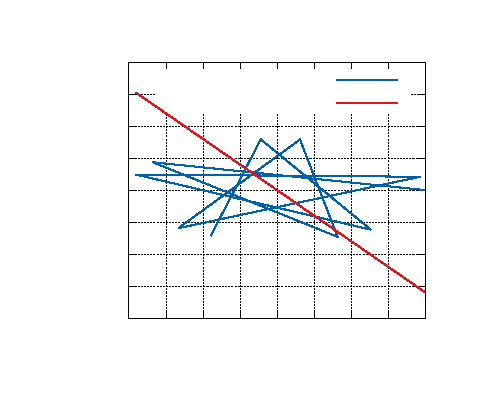
\includegraphics{sho10}}%
    \gplfronttext
  \end{picture}%
\endgroup
}
        \caption{$n=10$}
        \label{fig:sho10}
    \end{subfigure}
    \begin{subfigure}[b]{0.35\textwidth}
        \scalebox{.8}{% GNUPLOT: LaTeX picture with Postscript
\begingroup
  \makeatletter
  \providecommand\color[2][]{%
    \GenericError{(gnuplot) \space\space\space\@spaces}{%
      Package color not loaded in conjunction with
      terminal option `colourtext'%
    }{See the gnuplot documentation for explanation.%
    }{Either use 'blacktext' in gnuplot or load the package
      color.sty in LaTeX.}%
    \renewcommand\color[2][]{}%
  }%
  \providecommand\includegraphics[2][]{%
    \GenericError{(gnuplot) \space\space\space\@spaces}{%
      Package graphicx or graphics not loaded%
    }{See the gnuplot documentation for explanation.%
    }{The gnuplot epslatex terminal needs graphicx.sty or graphics.sty.}%
    \renewcommand\includegraphics[2][]{}%
  }%
  \providecommand\rotatebox[2]{#2}%
  \@ifundefined{ifGPcolor}{%
    \newif\ifGPcolor
    \GPcolortrue
  }{}%
  \@ifundefined{ifGPblacktext}{%
    \newif\ifGPblacktext
    \GPblacktextfalse
  }{}%
  % define a \g@addto@macro without @ in the name:
  \let\gplgaddtomacro\g@addto@macro
  % define empty templates for all commands taking text:
  \gdef\gplbacktext{}%
  \gdef\gplfronttext{}%
  \makeatother
  \ifGPblacktext
    % no textcolor at all
    \def\colorrgb#1{}%
    \def\colorgray#1{}%
  \else
    % gray or color?
    \ifGPcolor
      \def\colorrgb#1{\color[rgb]{#1}}%
      \def\colorgray#1{\color[gray]{#1}}%
      \expandafter\def\csname LTw\endcsname{\color{white}}%
      \expandafter\def\csname LTb\endcsname{\color{black}}%
      \expandafter\def\csname LTa\endcsname{\color{black}}%
      \expandafter\def\csname LT0\endcsname{\color[rgb]{1,0,0}}%
      \expandafter\def\csname LT1\endcsname{\color[rgb]{0,1,0}}%
      \expandafter\def\csname LT2\endcsname{\color[rgb]{0,0,1}}%
      \expandafter\def\csname LT3\endcsname{\color[rgb]{1,0,1}}%
      \expandafter\def\csname LT4\endcsname{\color[rgb]{0,1,1}}%
      \expandafter\def\csname LT5\endcsname{\color[rgb]{1,1,0}}%
      \expandafter\def\csname LT6\endcsname{\color[rgb]{0,0,0}}%
      \expandafter\def\csname LT7\endcsname{\color[rgb]{1,0.3,0}}%
      \expandafter\def\csname LT8\endcsname{\color[rgb]{0.5,0.5,0.5}}%
    \else
      % gray
      \def\colorrgb#1{\color{black}}%
      \def\colorgray#1{\color[gray]{#1}}%
      \expandafter\def\csname LTw\endcsname{\color{white}}%
      \expandafter\def\csname LTb\endcsname{\color{black}}%
      \expandafter\def\csname LTa\endcsname{\color{black}}%
      \expandafter\def\csname LT0\endcsname{\color{black}}%
      \expandafter\def\csname LT1\endcsname{\color{black}}%
      \expandafter\def\csname LT2\endcsname{\color{black}}%
      \expandafter\def\csname LT3\endcsname{\color{black}}%
      \expandafter\def\csname LT4\endcsname{\color{black}}%
      \expandafter\def\csname LT5\endcsname{\color{black}}%
      \expandafter\def\csname LT6\endcsname{\color{black}}%
      \expandafter\def\csname LT7\endcsname{\color{black}}%
      \expandafter\def\csname LT8\endcsname{\color{black}}%
    \fi
  \fi
    \setlength{\unitlength}{0.0500bp}%
    \ifx\gptboxheight\undefined%
      \newlength{\gptboxheight}%
      \newlength{\gptboxwidth}%
      \newsavebox{\gptboxtext}%
    \fi%
    \setlength{\fboxrule}{0.5pt}%
    \setlength{\fboxsep}{1pt}%
\begin{picture}(4320.00,3600.00)%
    \gplgaddtomacro\gplbacktext{%
      \csname LTb\endcsname%
      \put(946,704){\makebox(0,0)[r]{\strut{}$-2$}}%
      \csname LTb\endcsname%
      \put(946,1011){\makebox(0,0)[r]{\strut{}$-1.5$}}%
      \csname LTb\endcsname%
      \put(946,1318){\makebox(0,0)[r]{\strut{}$-1$}}%
      \csname LTb\endcsname%
      \put(946,1625){\makebox(0,0)[r]{\strut{}$-0.5$}}%
      \csname LTb\endcsname%
      \put(946,1932){\makebox(0,0)[r]{\strut{}$0$}}%
      \csname LTb\endcsname%
      \put(946,2238){\makebox(0,0)[r]{\strut{}$0.5$}}%
      \csname LTb\endcsname%
      \put(946,2545){\makebox(0,0)[r]{\strut{}$1$}}%
      \csname LTb\endcsname%
      \put(946,2852){\makebox(0,0)[r]{\strut{}$1.5$}}%
      \csname LTb\endcsname%
      \put(946,3159){\makebox(0,0)[r]{\strut{}$2$}}%
      \csname LTb\endcsname%
      \put(1078,484){\makebox(0,0){\strut{}$-0.4$}}%
      \csname LTb\endcsname%
      \put(1434,484){\makebox(0,0){\strut{}$-0.3$}}%
      \csname LTb\endcsname%
      \put(1789,484){\makebox(0,0){\strut{}$-0.2$}}%
      \csname LTb\endcsname%
      \put(2145,484){\makebox(0,0){\strut{}$-0.1$}}%
      \csname LTb\endcsname%
      \put(2501,484){\makebox(0,0){\strut{}$0$}}%
      \csname LTb\endcsname%
      \put(2856,484){\makebox(0,0){\strut{}$0.1$}}%
      \csname LTb\endcsname%
      \put(3212,484){\makebox(0,0){\strut{}$0.2$}}%
      \csname LTb\endcsname%
      \put(3567,484){\makebox(0,0){\strut{}$0.3$}}%
      \csname LTb\endcsname%
      \put(3923,484){\makebox(0,0){\strut{}$0.4$}}%
    }%
    \gplgaddtomacro\gplfronttext{%
      \csname LTb\endcsname%
      \put(176,1931){\rotatebox{-270}{\makebox(0,0){\strut{}Velocity/Acceleration}}}%
      \put(2500,154){\makebox(0,0){\strut{}Position}}%
      \csname LTb\endcsname%
      \put(2936,2986){\makebox(0,0)[r]{\strut{}Velocity}}%
      \csname LTb\endcsname%
      \put(2936,2766){\makebox(0,0)[r]{\strut{}Acceleration}}%
    }%
    \gplbacktext
    \put(0,0){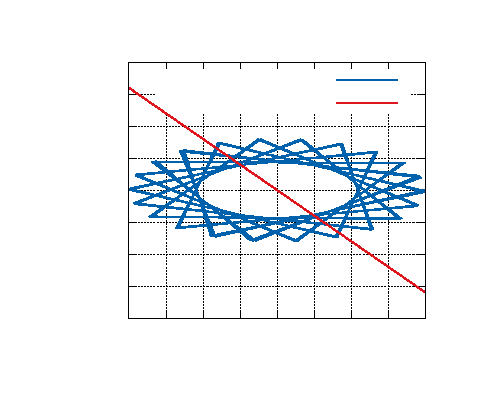
\includegraphics{sho50}}%
    \gplfronttext
  \end{picture}%
\endgroup
}
        \caption{$n=50$}
        \label{fig:sho50}
    \end{subfigure}
    \begin{subfigure}[b]{0.3\textwidth}
        \scalebox{.8}{% GNUPLOT: LaTeX picture with Postscript
\begingroup
  \makeatletter
  \providecommand\color[2][]{%
    \GenericError{(gnuplot) \space\space\space\@spaces}{%
      Package color not loaded in conjunction with
      terminal option `colourtext'%
    }{See the gnuplot documentation for explanation.%
    }{Either use 'blacktext' in gnuplot or load the package
      color.sty in LaTeX.}%
    \renewcommand\color[2][]{}%
  }%
  \providecommand\includegraphics[2][]{%
    \GenericError{(gnuplot) \space\space\space\@spaces}{%
      Package graphicx or graphics not loaded%
    }{See the gnuplot documentation for explanation.%
    }{The gnuplot epslatex terminal needs graphicx.sty or graphics.sty.}%
    \renewcommand\includegraphics[2][]{}%
  }%
  \providecommand\rotatebox[2]{#2}%
  \@ifundefined{ifGPcolor}{%
    \newif\ifGPcolor
    \GPcolortrue
  }{}%
  \@ifundefined{ifGPblacktext}{%
    \newif\ifGPblacktext
    \GPblacktextfalse
  }{}%
  % define a \g@addto@macro without @ in the name:
  \let\gplgaddtomacro\g@addto@macro
  % define empty templates for all commands taking text:
  \gdef\gplbacktext{}%
  \gdef\gplfronttext{}%
  \makeatother
  \ifGPblacktext
    % no textcolor at all
    \def\colorrgb#1{}%
    \def\colorgray#1{}%
  \else
    % gray or color?
    \ifGPcolor
      \def\colorrgb#1{\color[rgb]{#1}}%
      \def\colorgray#1{\color[gray]{#1}}%
      \expandafter\def\csname LTw\endcsname{\color{white}}%
      \expandafter\def\csname LTb\endcsname{\color{black}}%
      \expandafter\def\csname LTa\endcsname{\color{black}}%
      \expandafter\def\csname LT0\endcsname{\color[rgb]{1,0,0}}%
      \expandafter\def\csname LT1\endcsname{\color[rgb]{0,1,0}}%
      \expandafter\def\csname LT2\endcsname{\color[rgb]{0,0,1}}%
      \expandafter\def\csname LT3\endcsname{\color[rgb]{1,0,1}}%
      \expandafter\def\csname LT4\endcsname{\color[rgb]{0,1,1}}%
      \expandafter\def\csname LT5\endcsname{\color[rgb]{1,1,0}}%
      \expandafter\def\csname LT6\endcsname{\color[rgb]{0,0,0}}%
      \expandafter\def\csname LT7\endcsname{\color[rgb]{1,0.3,0}}%
      \expandafter\def\csname LT8\endcsname{\color[rgb]{0.5,0.5,0.5}}%
    \else
      % gray
      \def\colorrgb#1{\color{black}}%
      \def\colorgray#1{\color[gray]{#1}}%
      \expandafter\def\csname LTw\endcsname{\color{white}}%
      \expandafter\def\csname LTb\endcsname{\color{black}}%
      \expandafter\def\csname LTa\endcsname{\color{black}}%
      \expandafter\def\csname LT0\endcsname{\color{black}}%
      \expandafter\def\csname LT1\endcsname{\color{black}}%
      \expandafter\def\csname LT2\endcsname{\color{black}}%
      \expandafter\def\csname LT3\endcsname{\color{black}}%
      \expandafter\def\csname LT4\endcsname{\color{black}}%
      \expandafter\def\csname LT5\endcsname{\color{black}}%
      \expandafter\def\csname LT6\endcsname{\color{black}}%
      \expandafter\def\csname LT7\endcsname{\color{black}}%
      \expandafter\def\csname LT8\endcsname{\color{black}}%
    \fi
  \fi
    \setlength{\unitlength}{0.0500bp}%
    \ifx\gptboxheight\undefined%
      \newlength{\gptboxheight}%
      \newlength{\gptboxwidth}%
      \newsavebox{\gptboxtext}%
    \fi%
    \setlength{\fboxrule}{0.5pt}%
    \setlength{\fboxsep}{1pt}%
\begin{picture}(4320.00,3600.00)%
    \gplgaddtomacro\gplbacktext{%
      \csname LTb\endcsname%
      \put(946,704){\makebox(0,0)[r]{\strut{}$-2$}}%
      \csname LTb\endcsname%
      \put(946,1011){\makebox(0,0)[r]{\strut{}$-1.5$}}%
      \csname LTb\endcsname%
      \put(946,1318){\makebox(0,0)[r]{\strut{}$-1$}}%
      \csname LTb\endcsname%
      \put(946,1625){\makebox(0,0)[r]{\strut{}$-0.5$}}%
      \csname LTb\endcsname%
      \put(946,1932){\makebox(0,0)[r]{\strut{}$0$}}%
      \csname LTb\endcsname%
      \put(946,2238){\makebox(0,0)[r]{\strut{}$0.5$}}%
      \csname LTb\endcsname%
      \put(946,2545){\makebox(0,0)[r]{\strut{}$1$}}%
      \csname LTb\endcsname%
      \put(946,2852){\makebox(0,0)[r]{\strut{}$1.5$}}%
      \csname LTb\endcsname%
      \put(946,3159){\makebox(0,0)[r]{\strut{}$2$}}%
      \csname LTb\endcsname%
      \put(1078,484){\makebox(0,0){\strut{}$-0.4$}}%
      \csname LTb\endcsname%
      \put(1434,484){\makebox(0,0){\strut{}$-0.3$}}%
      \csname LTb\endcsname%
      \put(1789,484){\makebox(0,0){\strut{}$-0.2$}}%
      \csname LTb\endcsname%
      \put(2145,484){\makebox(0,0){\strut{}$-0.1$}}%
      \csname LTb\endcsname%
      \put(2501,484){\makebox(0,0){\strut{}$0$}}%
      \csname LTb\endcsname%
      \put(2856,484){\makebox(0,0){\strut{}$0.1$}}%
      \csname LTb\endcsname%
      \put(3212,484){\makebox(0,0){\strut{}$0.2$}}%
      \csname LTb\endcsname%
      \put(3567,484){\makebox(0,0){\strut{}$0.3$}}%
      \csname LTb\endcsname%
      \put(3923,484){\makebox(0,0){\strut{}$0.4$}}%
    }%
    \gplgaddtomacro\gplfronttext{%
      \csname LTb\endcsname%
      \put(176,1931){\rotatebox{-270}{\makebox(0,0){\strut{}Velocity/Acceleration}}}%
      \put(2500,154){\makebox(0,0){\strut{}Position}}%
      \csname LTb\endcsname%
      \put(2936,2986){\makebox(0,0)[r]{\strut{}Velocity}}%
      \csname LTb\endcsname%
      \put(2936,2766){\makebox(0,0)[r]{\strut{}Acceleration}}%
    }%
    \gplbacktext
    \put(0,0){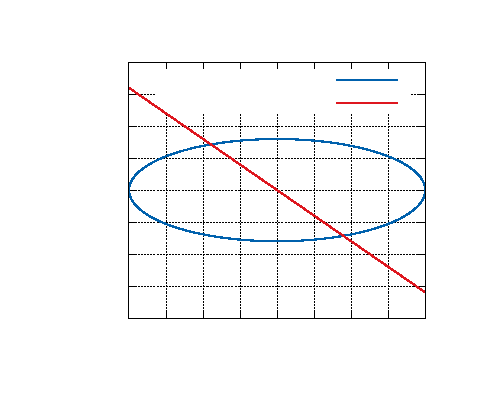
\includegraphics{sho1000}}%
    \gplfronttext
  \end{picture}%
\endgroup
}
        \caption{$n=1000$}
        \label{fig:sho1000}
    \end{subfigure}
    \caption{Simple harmonic oscillator plot smoothing as $n$ increases}\label{fig:sho}
\end{figure}

As $n \to \infty$, the shape of the velocity curve is much more clear. Interestingly, the
velocity is $0$ when displacement is maximum, and velocity is maximum when displacement is
$0$. The shape of the curve become much smoother with larger $n$, which is simply due to
the fact that we have more data points to represent the relationship.

\section{Conclusion}

We investigated the nature of errors when numerically computing derivatives. To the same conclusion
any student of elementary calculus could conclude, the gradient is much more accurate as $h \to 0$. Also, important
to note that depending on the data type we use (e.g. double vs. float) our precision will be affected. Generally speaking,
floats can store up to 7 decimals places, while doubles can store 15 decimals places. Hence, doubles have double the capacity
of floats, which explains the name.

For the simple harmonic oscillator experiment, the most important take away is to try to achieve as many data
points as permitted. However, computationally speaking as scientist we must also be savvy of our computational
bottlenecks. As data points increase, our precision might increase, yet our memory and processor consumption will
to. Thus, for later work such considerations can be explored and even quantified. While
investigating much experience was gained of using scientific computing tools such as gnuplot, Latex and C programming.

\begin{thebibliography}{9}

	\bibitem{lamport94}
	  Leslie Lamport,
	  \emph{\LaTeX: A Document Preparation System}.
	  Addison Wesley, Massachusetts,
	  2nd Edition,
	  1994.

  \bibitem{lamport94}
	  Andrew Roberts,
	  \emph{Getting to Grips with Latex}.
    http://www.andy-roberts.net/writing/latex

  \bibitem{lamport94}
	  ShareLaTex Documentation,
    http://www.andy-roberts.net/writing/latex

  \bibitem{lamport94}
	  Latex Wikibook.
    https://en.wikibooks.org/wiki/LaTeX

  \bibitem{lamport94}
	  C Data types,
    https://www.gnu.org/software/gnu-c-manual/gnu-c-manual.html#Real-Number-Types

\end{thebibliography}
\end{document}
